\documentclass[11pt]{article}
\usepackage[paperwidth=12cm, paperheight=18cm, margin=1cm]{geometry}
\usepackage{amsmath, tikz}
\pagestyle{empty}

\begin{document}
\begin{center}
  {\LARGE\bfseries The St.\ Petersburg Paradox}\\[4pt]
  {\large A game worth infinite money}
\end{center}

Flip a coin until it lands heads. If that takes \(k\) flips,
you win \(2^k\) dollars. How much would you pay to play?

\section*{The expected value is infinite}
\[
  E = \sum_{k=1}^{\infty} \frac{1}{2^k} \cdot 2^k
    = 1 + 1 + 1 + \cdots = \infty
\]

\begin{center}
\begin{tabular}{ccc}
  \hline
  Flips \(k\) & Probability & Prize \\
  \hline
  1 & 50\% & \$2 \\
  2 & 25\% & \$4 \\
  3 & 12.5\% & \$8 \\
  10 & 0.1\% & \$1024 \\
  \hline
\end{tabular}
\end{center}

\begin{center}
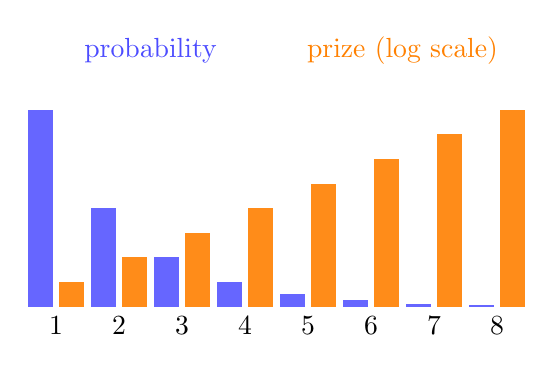
\begin{tikzpicture}[xscale=0.8, yscale=2.5]
  \foreach \k in {1, ..., 8} {
    \fill[blue!60] (\k-0.45,0) rectangle (\k-0.05, {1/2^\k * 2});
    \fill[orange!90] (\k+0.05,0) rectangle (\k+0.45, {\k/8});
    \node[below] at (\k,0) {\k};
  }
  \node[blue!70] at (2.5,1.3) {probability};
  \node[orange] at (6.5,1.3) {prize (log scale)};
\end{tikzpicture}
\end{center}

\section*{Bernoulli's answer: utility is logarithmic}
\[
  \sum_{k=1}^{\infty} \frac{\ln 2^k}{2^k} = 2 \ln 2
  \;\Rightarrow\; \text{fair price} \approx \$4
\]
\end{document}
